\section{Tectonic model}
\label{sec:tectonicmodel}
We now introduce the detailed description of the tectonic model used to create the planet crust. We discuss differences and similarities with respect to the original article and adapt the mechanisms to our unit sphere representation. Parameters that drive the model are summarized at the end of the section in Table \ref{tab:model-parameters-summary}. It should be stated that all parameters will be optimized for the number of vertex samples $N$ equal to 500,000.

The simplest description of the algorithm is that it creates some random crust partitioning into plates. These plates have randomized drifting parameters for moving. Then a certain number of tectonic steps is performed with a time step length $\delta t$ of 2 My and the result is a basic crust of the simulated planet. Between automated tectonic steps, user can force a few specific interactions (plate rifting, terrain smoothing) and change various global parameters to influence the simulation. The planet radius is set to $6370\mbox{ km}=6.37\mbox{ u}$.
\subsection{Workflow}
Basic crust is generated from a Delaunay triangulation of a unit sphere. The fresh crust is just a~set of triangulated vertices, while each vertex is assigned some default crust data $h$. Each tectonic step consists of several substeps in a sequence. This sequence is firmly set because of implementation context and is depicted in Figure \ref{fig:tectonic-step-structure}. Short descriptions for the substeps follow.
\begin{figure}[ht]
\centering
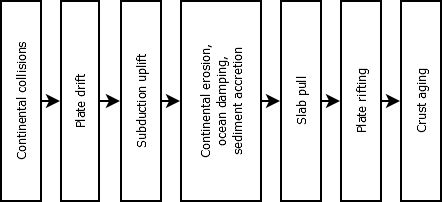
\includegraphics[width=12cm]{tectonic-step-structure.png}
\caption{Tectonic step structure}
\label{fig:tectonic-step-structure}
\end{figure}
\begin{itemize}[\label={}]
\item[\textbf{Continental collisions}] If the plate drift would result in an overlap of two different continental (above sea level) areas of crust belonging to different plates, a continental collision is triggered, resulting in a~massive uplift of the lighter plate. The two plates in question are then merged into one. This is different from the orignal algorithm, which only attaches connected continental areas, called \textit{terranes}.
\item[\textbf{Plate drift}] Rotation transform of each plate along the sphere surface is updated by its respective angular speed.
\item[\textbf{Subduction uplift}] Overlapping areas of different plates cause uplift in the lighter plates. This process is known as \textit{subduction}. Note that overlapping continental areas have already been dealt with so this case should never occur during this step.
\item[\textbf{Continental erosion, oceanic damping, sediment accretion}] This step updates elevation values to simulate erosion of crust above sea level, lowering of the ocean bottom for underwater crust and sediment accretion for the oceanic crust below average ocean depth. This is questionable, as the original algorithm probably detects trench area for sediment filling.
\item[\textbf{Slab pull}] Subducting parts of plates tend to pull the plate towards them, altering the surface rotation. All vertices in subduction zones contribute to the rotation vectors of their plates.
\item[\textbf{Plate rifting}] Every tectonic step the largest plate has a chance to rift apart. Along some random linear border within the plate the vertices are assigned to two new plates with diverging velocities.
\item[\textbf{Crust aging}] Age of every crust vertex is updated by the length of the tectonic step.
\end{itemize}
\subsection{Crust \& plates}
The crust is defined as a set of surface vertices $U$, obtained by Fibonacci sampling. Its size is the number of samples $N$. Each vertex $\mathbf{u}_i\in U$ is assigned crust point data $h_i$. The tectonic plate system is an~equivalence system $\mathcal{P}$ of $U$ (so that every crust point belongs exactly to one plate). These equivalence classes should be connected through the mesh, but it is not a strict requirement (although it subtracts from the realism). Plates are the individual equivalence classes $\mathcal{P}_i\in\mathcal{P}$. If all vertices of a~mesh triangle belong to a~plate $\mathcal{P}_i$, the triangle is also said to belong to $\mathcal{P}_i$. A triangle only has three neighbours, each sharing one edge. If a triangle belonging to $\mathcal{P}_i$ has a neighbouring triangle which does not, it is called a \textit{border triangle}.

Each plate is also assigned: a centroid $\mathbf{c}_i$, rotation axis $\mathbf{w}_i$, plate angular speed $\omega_i$ and a transform $q_i$. The centroid is a vector calculated as the normalized sum of all vector representations of vertices belonging to the plate. If it cannot be normalized, a random vector is assigned. The rotation axis is a unit vector along the axis around which the plate drifts. The plate angular speed is self-explanatory. The transform is a quaternion representation of the relative rotation of the plate with respect to the original position. This is because the simulation does not actually move the plate vertices, only adjusts the plate transform to correctly calculate interactions. Moving the vertices would introduce serious problems with rendering.
\subsection{Crust data}
Crust data values included so far are: elevation, crust thickness, orogeny type and crust age. All crust points are strictly represented by unit vectors. The elevation values are information stored separately. Oceanic crust are all crust points with negative elevation, continental crust points have a non-negative elevation. Crust thickness is a placeholder information for potential future updates. Orogeny type is represented by three categories: \textit{None}, \textit{Andean} and \textit{Himalayan}. The Andean type is a crust point elevated above the ocean level by subduction, the Himalayan type is a crust point that was influenced by continental collision. The None type is reserved for crust points not yet elevated by continental collision nor elevated above the ocean level by subduction. It does not exist in the original article, as the orogeny type is reserved for continental crust. The crust age is simple the time passed from the creation of the crust point. The original model also uses fold direction, which is not yet implemented, as I do not properly understand its purpose and mechanics.

The default crust point data for new points depends on whether the new point is continental or not. The only new continental points are created during the first partitioning (see Subsection \ref{subsec:plate-initialization}). Initial elevation is $z_{0t}=-0.004 \mbox{ u}$ for oceanic crust and $z_{0c}=0.001 \mbox{ u}$ for continental crust. Crust thickness is always calculated from a~basic crust thickness value $e_0=0.01\mbox{ u}$ as $e=e_0+z$, where $z$ is the crust elevation. The initial orogeny type is None for all new oceanic crust points and Andean for the initial continental crust. Initial crust age is universally equal to 0.
\subsection{Plate initialization}
\label{subsec:plate-initialization}
Partitioning of the crust into the initial set of plates  is governed by two parameters: the number of initial plates $N_\mathcal{P}$ and the probability of an initial plate being continental $p_C$. The initial number of plates is 20 and the probability of an initial plate to be continental is 0 for testing purposes. Before partitioning, vector noise is assigned to each triangle on the mesh with a noise averaging iterations parameter $n_{\mbox{sm}}$ of 4.

At first, $N_\mathcal{P}$ number of random points $\mathbf{c}$ (future \textit{centroids} of the plates) is distributed on the surface. Then all initial crust vertices are assigned to these points by their shortest distance on a unit sphere:
$$d(\mathbf{x},\mathbf{c})=\arccos(\mathbf{x}\cdot\mathbf{c})$$
All points that have the shortest distance to a certain centroid point belong to a single plate. This plate inherints the points and the centroid. When all points are distributed to their plates, each plate is then assigned a random rotation axis $\mathbf{w}$ and random non-negative angular speed $\omega$. The maximum plate angular speed is $v_0=0.0157\mbox{ My}^{-1}$. The symbol is unchanged to correspond with the original quantity. Finally, each plate is assigned a quaternion identity transform $q$. All crust points are assigned default data according to their plate. The probability of continental crust is evaluated on the plate level, so the initial plates all have the same elevation.

This kind of initialization basically creates a Voronoi diagram with perfectly straight lines (up to the triangle resolution). To simulate more realistic plate boundaries, vector noise is used. First we look for the triangles which have vertices from exactly two different plates. For each of these triangles we try to roll for probability equal to its noise vector magnitude. If the probability succeeds, we compute three dot products between the noise vector and each vector from the triangle barycenter to the vertex. The vertex with the maximum dot product is assigned to the plate of the vertex with the minimum dot product. This shifts the borders of the plates and is repeated $n_{\mbox{vb}}=4$ times. This parameter is the number of Voronoi border shift iterations. An example of the resulting partitioning can be seen in Figure \ref{fig:initial-plates}.
\begin{figure}[ht]
\centering
\begin{subfigure}{7cm}
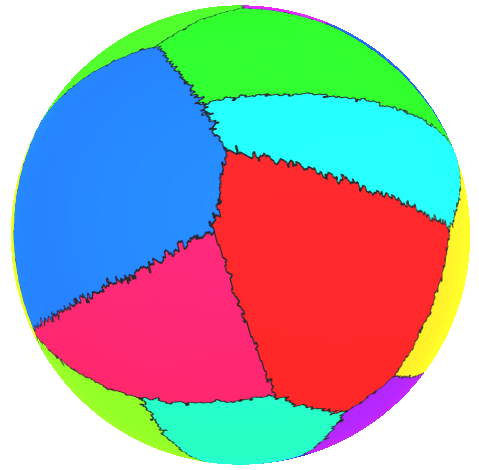
\includegraphics[height=7cm]{plate-initialization.png}
\caption{initial plates}
\label{fig:initial-plates}
\end{subfigure}
\hspace*{1cm}
\begin{subfigure}{7cm}
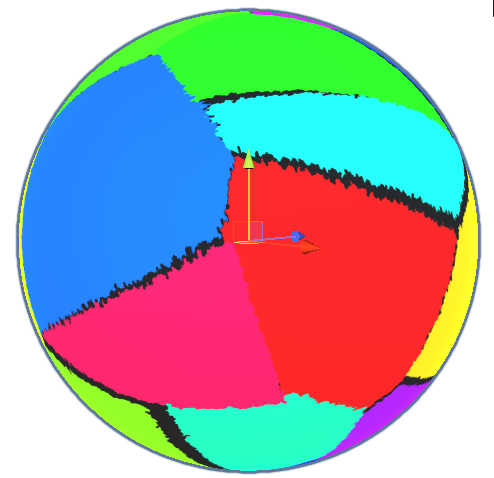
\includegraphics[height=7cm]{plate-drift.png}
\caption{plates drifting}
\label{fig:plates-drifting}
\end{subfigure}
\caption{Crust partitioning}
\label{fig:crust-partitioning}
\end{figure}
\subsection{Plate overlaps}
Tectonic interactions require the concept of plate density. For example, denser oceanic plates are subducted under continental plates. Because our model does not have a clear designation of a plate as oceanic or continental (any plate can have oceanic or continental crust), we evaluate plates by a weighted sum of their vertices. Each plate is assigned a score equal to:
$$\mbox{score}=100\times\mbox{number of continental crust points}-\mbox{number of oceanic crust points}$$
The plates are then ranked by the highest score. The rank decides which plate 'goes under' when two plates overlap (the one with a lower score). This actually creates an irreflexive, antisymmetric and transitive relation on the set of plates.

This ranking system is a gross simplification. As many simplifications, though, it makes certain decisions and calculations much easier. The plate ranks have to be recalculated every time an interaction requires them, as the scores change both with crust elevation and changes in crust point assignments to plates. An example might be when we need to know which of the overlapping plates defines a crust point elevation on the surface.
\subsection{Plate drift}
The main reason for tectonic interactions is the tectonic drift. Plates move constantly, causing collisions, subduction etc. To model the drift of a plate, during every tectonic step the plate transform is adjusted
by multiplication of the transform by a quaternion representing a rotation around the axis $\mathbf{w}$ by the angle of $\Delta\phi=\omega\delta t$. This keeps the information about current crust points locations. The result of a one step drift from the initial position can be seen in Figure \ref{fig:plates-drifting}. We can see here that the plates move as individual rigid bodies.
\subsection{Oceanic crust generation \& crust resampling}
Moving rigid plates necessarily create gaps on the surface. In reality, this 'empty' space is filled with new crust drifting from oceanic ridges between the plates (see Figure \ref{fig:resample-mesh}). We use the original model, only slightly simplified. We can interpolate crust data at any point on the surface which is not in any triangle belonging to a plate. We compute two distances to two nearest plates (nearest vertices belonging to two different plates) $d_1$ and $d_2$ (1 being the absolute shortest) and assume that the point is approximately on the direct line between the nearest points. We also assume that the ridge is directly in the middle of the line. This is not true in reality, but makes it simple to use the original algorithm easily. We compute the ridge and plate elevation contributions and combine them as per Cortial et al.
\begin{figure}[ht]
\centering
\begin{subfigure}{7cm}
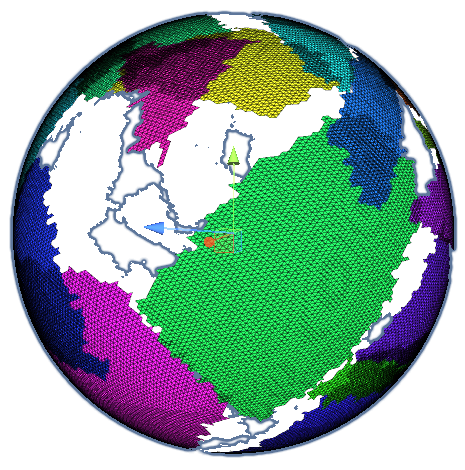
\includegraphics[height=7cm]{resample-drift.png}
\caption{diverging plates}
\label{fig:resample-drift}
\end{subfigure}
\hspace*{1cm}
\begin{subfigure}{7cm}
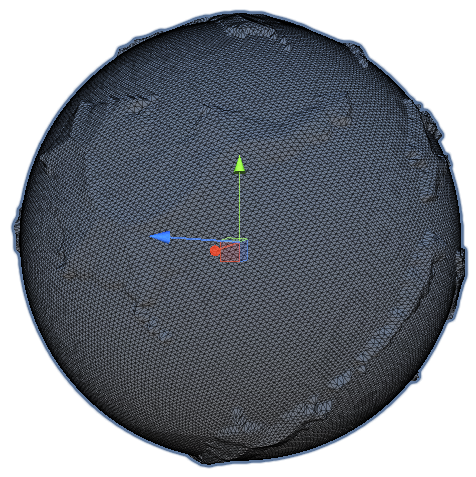
\includegraphics[height=7cm]{resample-ridges.png}
\caption{generated ridges}
\label{fig:resample-ridges}
\end{subfigure}
\caption{Oceanic crust generation}
\label{fig:resample-mesh}
\end{figure}

The ridge function profile uses three parameters: the highest oceanic ridge elevation $z_r$, the abyssal plains elevation $z_a$ and the oceanic ridge elevation falloff $\sigma_r$. The values of these parameters are:
$$z_r=-1\mbox{ km}=-0.001\mbox{ u}$$
$$z_a=-6\mbox{ km}=-0.006\mbox{ u}$$
$$\sigma_r=0.05\mbox{ u}$$
The ridge function profile is a function of a variable $d_\Gamma$ which is the distance to the oceanic ridge. The function profile is chosen as:
$$z_\Gamma=(z_r-z_a)2^{\frac{d_\Gamma}{\sigma_r}}+z_a$$
The original function profile is not specifically described and may be more complex.
Because of our assumptions we can calculate the ridge function profile variable that is the distance to the ridge as:
$$d_\Gamma=\frac{d_2-d_1}{2}$$
The orogeny type is universally filled as None for points in the surface voids. The crust age is computed as the scaling parameter $\alpha=\frac{d_\Gamma}{d_\Gamma+d_1}$ multiplied by the total time for which the plates have been diverging (since last they were in close contact). This makes the new oceanic crust gradually older the further it is from the ridge. Finally, any new oceanic crust point is assigned to the nearest plate.

For simulation running for many steps it is vital that we periodically resample the surface to fill the gaps made by diverging plates and to resolve overlapping plates. As per Cortial et al., it is recommended to resample the surface every 10th-60th step. Our model forces resampling on several occasions, namely continental collision. The resampling simply means to interpolate surface data onto the original mesh from the current surface data defined on a mesh broken by drifting plates and interactions. For each initial mesh vertex, we test if it is found on a plate with the highest rank possible. If so, we perform barycentric interpolation from a triangle within which the vertex currently resides. If no plate is found, we create a new oceanic crust point. When all crust point data is assigned, the original mesh with the interpolated crust point data becomes the new crust model. Because the algorithm remembers to which plates the crust points belong, the new crust points are reassigned to their respective plates and the plate transforms are reset to identity.

\subsection{Continental collisions}
The quaternion transform mechanics have both advantages and disadvantages. The main advantage is that it allows for faster computations and relatively simple data management. The main disadvantage is that it does not allow for simple crust point reassignment to another plate if the plates' respective transforms are not identities. For this reason, whenever a point is assigned to another plate, a resample must be performed in advance. This is the reason why continental collisions are evaluated as the very first in a tectonic step. We use a predictive detection, that is we first simulate a one-step drift and then detect whether two continental triangles (triangles with all-continental points) from two different plates intersect. This is sufficient condition for triggering a continental collision. This varies significantly from Cortial et al. because we do not require the plates to overlap over a specific distance (the 300 km and more originally). This may create unwanted tectonic artifacts and should be addressed in the future. Note that the simulated drift does not actually move the plates, it only adjusts transforms for the collision tests.

First we test all continental triangles for continental collisions with all other plates and store all collision triggers. If any such trigger occurs, we first flag all vertices in the triggering triangles and then we search for all connected groups of continental vertices that contain the flagged vertices and belong to a~single plate. These groups are called \textit{terranes}. It should be noted here that it is theoretically possible for one triangle to be colliding with two different plates. When constructing terranes, we only accept the first matching plate in order. This order is arbitrary and only depends on the order in which the plates are stored in the memory. Multi-collision for terranes is therefore ignored, as it is a very rare occurence. The way terranes are constructed allow for a vertex to be flagged as colliding with a plate with which it was not flagged as colliding beforehand, simply because it belongs to a single terrane from a vertex which does. Although this is not based on reality, it does make the algorithm unambiguous and hopefully does not negatively affect the simulation. If a continental collision occured, we now perform a one-step drift for all plates.

We now have a set of terranes belonging to certain plates. Each terrane has an assigned plate with which it collides. All terranes have a radius of influence inside which they cause collision uplift. This radius depends on several parameters. The first is the global maximum collision distance $r_c$, the second is the relative plate speed $v_{ij}$ at the terrane centroid, the third is the maximum plate speed $v_0$, the fourth is the area of the terrane $\mathcal{A}_i$ and the fifth is the average initial plate area $\mathcal{A}_0$. The global maximum collision distance is a model parameter, which needs to be scaled to the unit sphere:
$$r_c=\frac{4200\mbox{ km}}{6.37\mbox{ u}}=\frac{4.2\mbox{ u}}{6.37\mbox{ u}}\approx 0,659$$
The vector velocity of a plate $\mathcal{P}_i$ at a certain point $\mathbf{q}\in\mathcal{S}$ is equal to:
$$\mathbf{s}_i(\mathbf{q})=\omega_i\mathbf{w}_i\times\mathbf{q}$$
Relative speed of two plates $\mathcal{P}_i,\mathcal{P}_j$ at a point $\mathbf{q}$ is:
$$v_{ij}(\mathbf{q})=||\mathbf{s}_i(\mathbf{q})-\mathbf{s}_j(\mathbf{q})||=||\omega_i\mathbf{w}_i\times\mathbf{q}-\omega_j\mathbf{w}_j\times\mathbf{q}||=||(\omega_i\mathbf{w}_i-\omega_j\mathbf{w}_j)\times\mathbf{q}||$$
The radius of influence is computed as follows:
$$r = r_c\min(\xi,1), \xi = \sqrt{\frac{v_{ij}}{v_0}}\frac{\mathcal{A}_i}{\mathcal{A}_0}\approx \sqrt{\frac{v_{ij}}{v_0}}N_i\frac{N_\mathcal{P}}{N}= \sqrt{\frac{v_{ij}}{v_0}}\frac{N_i}{N_0}$$
The ratio of terrane area to the average initial area is approximately the same as the ratio of the number of terrane vertices to the average number of vertices in an initial plate, provided the number of samples is sufficiently high. The minimum value sets absolute maximum collision distance to prevent extreme elevation changes across continents for large mass collisions.

This range applies to area beyond the border of the terrane. A vertex on a plate in which the terrane collides is affected by the collision uplift if its distance $d$ from the nearest vertex of the terrane is less or equal to $r$.

If  a crust point is affected by a continental collision, this collision causes an immediate uplift based on a discrete collision coefficient $\Delta_c=1.3\times10^{-5}\mbox{ km}^{-1}=1.3\times10^{-2}\mbox{ u}^{-1}$. The uplift is is computed as follows:
$$\Delta z_i=\Delta_c\mathcal{A}_i\left(1-\left(\frac{d}{r}\right)^2\right)^2\approx4\pi R^2\frac{N_i}{N_\mathcal{P}}\Delta_c\left(1-\left(\frac{d}{r}\right)^2\right)^2,d\in[0,r]$$
This value is added to the elevation value of the crust point. If a crust point was affected by a~continental collision, its orogeny type becomes Himalayan. Finally, after all collisions have been resolved, we resample the whole crust, the vertices of all colliding terranes are reassigned to their new plates and the whole crust is resampled again.
\subsection{Subduction uplift}
The process of subduction takes place when two plates come into contact and continental collision is not triggered. Continental collisions should already be dealt with when subduction is evaluated. If the plates did not drift during a continental collision event, a one-step plate drift is performed before testing subduction events.

Subduction test begins with determining all subduction front points. Given a border triangle $\mathcal{T}_i$ on a~plate $\mathcal{P}_i$, we search all other plates for triangles intersecting with $\mathcal{T}_i$. For each other plate, we try to find at least one and take the first. If such a triangle $\mathcal{T}_j$ is found on a plate $\mathcal{P}_j$, we store a~new subduction front point at the the centroid location $\mathbf{c}_i$ of $\mathcal{T}_i$ assigned to $\mathcal{P}_i$ with the subduction uplift source $\mathcal{P}_j$ and an elevation value equal to the mean elevation value of the vertices in $\mathcal{T}_j$ . We try to find a~subduction front point for all border triangles on all plates.

Subduction front point information is then used to calculate the potential subduction uplift for all crust vertices. For each crust vertex $\mathbf{p}_i$ and each of its possible subduction uplift source plates, we find the smallest distance $d_j$ to a~subduction front point assigned to its plate with a given subduction source plate $\mathcal{P}_j$. There is a maximum distance allowed for subduction, called \textit{maximum subduction distance} $r_s$. Our model value is:
$$r_s=\frac{1800\mbox{ km}}{6.37\mbox{ u}}=\frac{1.8\mbox{ u}}{6.37\mbox{ u}}\approx0.283$$
If the subduction uplift source plate $\mathcal{P}_j$ has a lower overlap score $d_j<r_s$, we calculate the subduction uplift contribution, otherwise the contribution is set to 0.\footnote{We also set the contribution to 0 if there is no subduction front point for a given subduction uplift source plate.} The uplift contribution $\tilde{u}_j$ from $\mathcal{P}_j$ has three parts: distance transfer, speed transfer and height transfer:
$$ \tilde{u}_j=u_0 u_{\mbox{\small{dt}}}u_{\mbox{\small{st}}}u_{\mbox{\small{ht}}}$$

$u_0=0.6\mbox{ mm}\cdot\mbox{y}^{-1}=0.0006\mbox{ u}\cdot\mbox{My}^{-1}$ is called \textit{base subduction uplift}. The distance transfer is a~parametrized cubic function:\footnote{Cortial et al. only mention piece-wise cubic function, this is an example implementation.}
$$u_{\mbox{\small{dt}}}(d_j)=\frac{\frac{d_j^3}{3}-\frac{(r_c+r_s)d_j^2}{2}+r_cr_sd_j+\frac{r_s^3}{6}-\frac{r_s^2r_c}{2}}{\frac{r_s^3-r_c^3}{6}+\frac{r_c^2r_s-r_s^2r_c}{2}}$$
$r_c=0.1$ is the \textit{subduction control distance} and it is the distance in which the transfer has maximum. The other transfer functions are computed as follows:
$$u_{\mbox{\small{st}}}(v_{ij})=\frac{v_{ij}(\mathbf{p}_i)}{v_0},u_{\mbox{\small{ht}}}(z_j)=\left(\frac{z_j-z_t}{z_c-z_t}\right)^2$$
$v_{ij}$ is the relative speed plate at $\mathbf{p}_i$ and $z_j$ is the elevation value of the subduction front point.

When all uplift contributions $\tilde{u}_j$ have been calculated at $\mathbf{p}_i$ for all possible subduction uplift source plates $\mathcal{P}_j$, the vertex elevation $z_i$ is increased by:
$$\Delta z_i=\delta t\sum_j \tilde{u}_j$$
The subduction event possibly differs from Cortial et al. in that multiple contributions are possible at once and also the height transfer is carried from the subduction front as opposed to the original expression (denoted $z_i(\mathbf{p})$ in the article). This algorithm, however, presented no observed artifacts so far. It should be noted, however, that terranes on a mostly oceanic plate get subducted under an oceanic plate with a higher overlap score -- this, apparently, is not very realistic.
\subsection{Continental erosion}
The continental crust erosion adjusts the elevation values of all continental crust points:
$$\Delta z = -\frac{z}{z_c}\epsilon_c\delta t$$
$\epsilon_c=3\times10^{-2}\mbox{ mm}\cdot\mbox{y}^{-1}=3\times10^{-5}\mbox{ u}\cdot\mbox{My}^{-1}$ is the \textit{continental erosion parameter}.
\subsection{Oceanic damping}
The oceanic damping adjusts the elevation values of all oceanic crust points:
$$\Delta z = -\left(1-\frac{z}{z_t}\right)\epsilon_o\delta t$$
$\epsilon_o=4\times10^{-2}\mbox{ mm}\cdot\mbox{y}^{-1}=4\times10^{-5}\mbox{ u}\cdot\mbox{My}^{-1}$ is the \textit{oceanic damping parameter}.
\subsection{Sediment accretion}
The sediment accretion adjusts the elevation values of all oceanic crust points below the average ocean depth $\bar{z}_{o}=-0.004\mbox { u}$:
$$\Delta z = \epsilon_t\delta t$$
$\epsilon_t=3\times10^{-1}\mbox{ mm}\cdot\mbox{y}^{-1}=3\times10^{-4}\mbox{ u}\cdot\mbox{My}^{-1}$ is the \textit{sediment accretion parameter}.
\subsection{Slab pull}
All vertices of a plate $\mathcal{P}_i$ in a subduction front of another plate $\mathcal{P}_j$ alter its rotation axis $\mathbf{w}_i$. In our model, this means we have to flag all vertices that are found inside any triangle belonging to another plate with a higher overlap score. Again, we assume no continental collision is taking place since all such events have been resolved earlier in the tectonic step. We group all vertices by the plates they belong to and then we compute slab pull contributions for each plate. Given a plate $\mathcal{P}_i$ with a~rotation axis $\mathbf{w}_i$ and a~centroid $\mathbf{c}_i$, the slab pull adjustment for $n$ flagged points (each at a~location $\mathbf{q}_k$) is computed as follows:
$$\delta\mathbf{w}_i=\epsilon'\sum_{k=0}^{n-1}\frac{\mathbf{c}_i\times\mathbf{q}_k}{||\mathbf{c}_i\times\mathbf{q}_k||}\delta t$$
$\epsilon'$ is a perturbation coefficient scaling the influence of the slab pull. Because the summation vector varies wildly with the total number of mesh vertices, we need to find a~parameter somewhat independent of $N$. We chose $\epsilon'=\epsilon\frac{N_\mathcal{P}}{N}$ and call the new parameter $\epsilon=0.1$ \textit{slab pull perturbation parameter}. After the adjustments are computed for all plates, they are added as vectors to their respective axes and the results are normalized to 1.
\subsection{Plate rifting}
Continental collisions inevitably create unproportionally large tectonic plates. This leads to decreased tectonic activity and created continents sink through erosion into the ocean. To counter that, there is a~chance for plates to rift. Every tectonic step Driftworld checks probability to rift the largest plate.\footnote{The original article does not mention the mechanism specifically, but it probably checks all plates.} The probability for a plate $\mathcal{P}_j$ to rift is $p_i=\lambda_i e^{-\lambda_i}$. Driftworld computes the parameter $\lambda_i$ differently as:
$$\lambda_i=\lambda_0\frac{\mathcal{A}_i}{\mathcal{A}_0}\delta t=\lambda_0\frac{N_iN_\mathcal{P}}{N}\delta t$$
$\lambda_0=0.1\mbox{ My}^{-1}$ is the \textit{average rifting frequency}.

If the rifting event is triggered, the plate is divided into two plates by two random centroids within the plate according to the closest vertex distance. Finally, vector noise is applied to the shared border.
\subsection{Crust aging}
All crust points age is simply incremented by $\delta t$.
\begin{table}[h]
\centering
\begin{tabular}{cccc}
\textbf{Symbol}&\textbf{Description}&\textbf{Original value}&\textbf{Model value}\\
\hline
$N$&Number of mesh vertices&-&500,000\\
$\delta t$&Tectonic time step&2 My&2 My\\
$R$&Planet radius&6,378 km&6.37 u\\
$z_{0t}$&Initial oceanic elevation&-&-0.004 u\\
$z_{0c}$&Initial continental elevation&-&0.001 u\\
$e_0$&Basic crust thickness&-&0.01 u\\
$N_\mathcal{P}$&Initial number of plates&40&20\\
$p_C$&Initial continental plate probability&0.3&0\\
$v_0$&Maximum plate speed&100 mm$\cdot$y$^{-1}$&$0.0157\mbox{ My}^{-1}$\\
$n_{\mbox{sm}}$&Noise averaging iterations&-&4\\
$n_{\mbox{vb}}$&Voronoi border shift iterations&-&4\\
$z_r$&Highest oceanic ridge elevation&$-1\mbox{ km}$&$-0.001\mbox{ u}$\\
$z_a$&Abyssal plains elevation&-6\mbox{ km}&$-0.006\mbox{ u}$\\
$\sigma_r$&Oceanic ridge elevation falloff&-&$0.05$\\
$r_c$&Maximum global collision distance&4200 km&0.659\\
$\Delta_c$&Discrete collision coefficient&$1.3\times10^{-5}\mbox{ km}^{-1}$&$1.3\times10^{-2}\mbox{ u}^{-1}$\\
$r_s$&Maximum subduction distance&1800 km&0.283\\
$u_0$&Base subduction uplift&$0.6\mbox{ mm}\cdot\mbox{y}^{-1}$&$0.0006\mbox{ u}\cdot\mbox{My}^{-1}$\\
$r_c$&Subduction control distance&-&0.1\\
$\epsilon_c$&Continental erosion parameter&$3\times10^{-2}\mbox{ mm}\cdot\mbox{y}^{-1}$&$3\times10^{-5}\mbox{ u}\cdot\mbox{My}^{-1}$\\
$\epsilon_o$&Oceanic damping parameter&$4\times10^{-2}\mbox{ mm}\cdot\mbox{y}^{-1}$&$4\times10^{-5}\mbox{ u}\cdot\mbox{My}^{-1}$\\
$\bar{z}_o$&Average ocean depth&-&-0.004 u\\
$\epsilon_t$&Sediment accretion parameter&$3\times10^{-1}\mbox{ mm}\cdot\mbox{y}^{-1}$&$3\times10^{-4}\mbox{ u}\cdot\mbox{My}^{-1}$\\
$\epsilon$&Slab pull perturbation parameter&-&0.1\\
$\lambda_0$&Average rifting frequency&-&$0.1\mbox{ My}^{-1}$\\
\end{tabular}
\caption{Model parameters summary}
\label{tab:model-parameters-summary}
\end{table}